\section{Literature Review}

\subsection{Diagnosis and Management of Symptoms with Aid of Computers}

With the advent and distribution of personal computing devices, previous studies have explored and proposed various computer-based techniques that supports diagnosis of various diseases and disorders. For example, Shin and his colleagues TalkingBoogie, a mobile app that supports ad hoc notes of communicative issues that children with non-verbal developmental disabilities show~\cite{shin2020talkingboogie}. Salai and Baillie developed a mobile application for recording overactive bladder symptoms~\cite{salai2019wee}.

\subsection{Age-related Macular Degeneration (AMD)}

\subsubsection{Distortion}

\begin{figure}[h!]
    \centering
    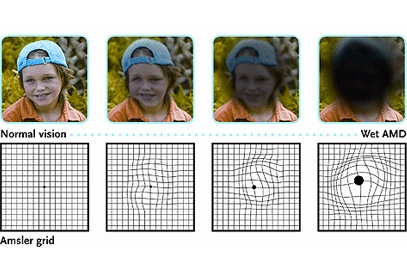
\includegraphics[width=0.6\linewidth]{figure/symptoms.jpg}
    \caption{Distortion}
    \label{fig:my_label}
\end{figure}

\subsection{Computer-based AMD Diagnosis}

Previous studies in the field of Human-computer interaction, bioengineering, and health informatics have explored several techniques that support medical practitioners and patients to diagnose symptoms of AMD in computers. Noting that paper-based AMD testing had been shown unsuccessful in terms of precise diagnosis~\cite{fine1986earliest, roy1985vision}, these studies emphasized the feasibility of computer-based approach for the precise and quantitative report of symptoms.

For example, Loewenstein et al. proposed MCPT, a system that supports patients to draw their region of symptoms on the computer~\cite{loewenstein2003replacing}. With basic input sources such as ordinary mouse and keyboard, these researchers sought to support a precise computer-based diagnosis. Mohaghegh and his colleagues developed a wearable system for diagnosing AMD symptoms~\cite{mohaghegh2016wearable}. They developed NGRID, a diagnosis system with a head-mounted device to support more precise diagnosis of AMD. In addition to such approaches, recent advent of 3D technologies made it possible to diagnose with 3D screen and glasses~\cite{kim2020novel}.

\begin{table}[htbp]
	\begin{center}
		\begin{tabular}{|c|c|} \hline
			Name & Description\\ \hline
			\hline {\sc MCPT~\cite{loewenstein2003replacing}} & Drawing on the computer with ordinary mouse and keyboard\\
			\hline {\sc NGRID~\cite{mohaghegh2016wearable}} & Head-mounted Amsler-grid app\\
			\hline {\sc 3D Test~\cite{kim2020novel}} & Implemented with 3D screen and polarized glasses\\
			\hline
		\end{tabular}
		\caption{Examples of AMD Diagnosis apps}
		\label{tab1}
	\end{center}
\end{table}

As such, previous researchers were successful in exploring design spaces of novel diagnosis systems and proposing them. Yet, these approaches are limited in its efficiency and generalizability, since (i) they only made use of simple input devices that might not be sufficient in terms of accuracy or (ii) the techniques required costly devices that are not easily available. With recent distribution of touch-based tablets, I found that these devices might give people a great opportunity to precisely note regions of symptom without purchasing any costly device. Thus, in this study, I propose an AMD diagnosis app that lets users easily utilize within their hand-held devices.